\subsection{x86}

\subsubsection{x86 + MSVC}

\RU{Имеем в итоге функцию \TT{f\_signed()}:}\EN{Here is how the \TT{f\_signed()} function looks like:}

\lstinputlisting[caption=\NonOptimizing MSVC 2010]{patterns/07_jcc/simple/signed_MSVC.asm}

\index{x86!\Instructions!JLE}
\RU{Первая инструкция \JLE значит}
\EN{The first instruction, \JLE, stands for} \IT{Jump if Less or Equal}. 
\RU{Если второй операнд больше первого или 
равен ему, произойдет переход туда, где будет следующая проверка.}
\EN{In other words, if the second operand is 
larger or equal to the first one, the control flow will be passed to the specified in the instruction address or label.}
\RU{А если это условие не срабатывает (то есть второй операнд меньше первого), то перехода не будет, 
и сработает первый \printf.}
\EN{If this condition does not trigger because the second operand is smaller than the first one, the control flow would not be altered and the first \printf would be executed.}
\index{x86!\Instructions!JNE}
\RU{Вторая проверка это}\EN{The second check is} \JNE: \IT{Jump if Not Equal}.
\RU{Переход не произойдет, если операнды равны}\EN{The control flow will not change if the operands are 
equal}.

\index{x86!\Instructions!JGE}
\RU{Третья проверка}\EN{The third check is} \JGE: \IT{Jump if Greater or Equal}\EMDASH{}\RU{переход 
если первый операнд больше второго или равен ему}\EN{jump if the first operand is larger than 
the second or if they are equal}.
\RU{Кстати, если все три условных перехода сработают, ни один \printf не вызовется. 
Но без внешнего вмешательства это невозможно.}
\EN{So, if all three conditional jumps are triggered, none of the \printf calls would be executed whatsoever. 
This is impossible without special intervention.}

\EN{Now let's take a look at the \TT{f\_unsigned()} function.}
\EN{The}\RU{Функция} \TT{f\_unsigned()} \RU{точно такая же, за тем исключением, что используются инструкции 
\JBE и \JAE вместо \JLE и \JGE:}
\EN{function is the same as \TT{f\_signed()}, with the exception that the \JBE and \JAE instructions
are used instead of \JLE and \JGE, as follows:}

\lstinputlisting[caption=GCC]{patterns/07_jcc/simple/unsigned_MSVC.asm}

\index{x86!\Instructions!JBE}
\index{x86!\Instructions!JAE}
\RU{Здесь всё то же самое, только инструкции условных переходов немного другие:}
\EN{As already mentioned, the branch instructions are different:}
\JBE\EMDASH{}\IT{Jump if Below or Equal} \AndENRU \JAE\EMDASH{}\IT{Jump if Above or Equal}.
\RU{Эти инструкции}\EN{These instructions} (\JA/\JAE/\JB/\JBE) 
\RU{отличаются от}\EN{differ from} \JG/\JGE/\JL/\JLE \RU{тем, что работают с беззнаковыми переменными.}
\EN{in the fact that they work with unsigned numbers.}

\index{x86!\Instructions!JA}
\index{x86!\Instructions!JB}
\index{x86!\Instructions!JG}
\index{x86!\Instructions!JL}
\index{Signed numbers}
\RU{Отступление: смотрите также секцию о представлении знака в числах}
\EN{See also the section about signed number representations}~(\myref{sec:signednumbers}).
\RU{Таким образом, увидев где используется \JG/\JL вместо \JA/\JB и наоборот, 
можно сказать почти уверенно насчет того, 
является ли тип переменной знаковым (signed) или беззнаковым (unsigned).}
\EN{That is why if we see \JG/\JL in use instead of \JA/\JB or vice-versa, 
we can be almost sure that the variables are signed or unsigned, respectively.}

\RU{Далее функция \main, где ничего нового для нас нет:}
\EN{Here is also the \main function, where there is nothing much new to us:}

\lstinputlisting[caption=\main]{patterns/07_jcc/simple/main_MSVC.asm}

\ifdefined\IncludeOlly
\clearpage
\subsubsection{x86 + MSVC + \olly}
\index{\olly}
\index{x86!\Registers!\Flags}

\RU{Если попробовать этот пример в \olly, можно увидеть, как выставляются флаги}\EN{We
can see how flags are set by running this example in \olly}.
\RU{Начнем с ф-ции}\EN{Let's begin with} \TT{f\_unsigned()}\RU{, которая работает с беззнаковыми числами}
\EN{, which works with unsigned numbers}.
\RU{В целом, в каждой ф-ции, \CMP исполняется три раза, но для одних и тех же аргументов, 
так что флаги все три раза будут одинаковы.}
\EN{\CMP is executed thrice here, but for the same arguments, 
so the flags are the same each time.}

\RU{Результат первого сравнения}\EN{Result of the first comparison}:

\begin{figure}[H]
\centering
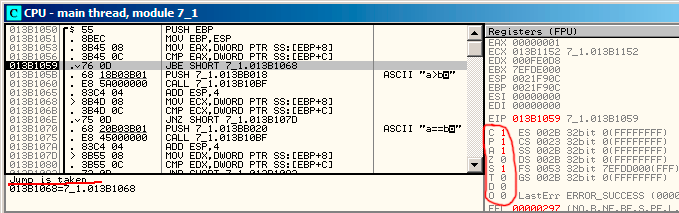
\includegraphics[scale=\FigScale]{patterns/07_jcc/simple/olly_unsigned1.png}
\caption{\olly: \TT{f\_unsigned()}: \RU{первый условный переход}\EN{first conditional jump}}
\label{fig:jcc_olly_unsigned_1}
\end{figure}

\RU{Итак, флаги}\EN{So, the flags are}: C=1, P=1, A=1, Z=0, S=1, T=0, D=0, O=0.
\RU{Для краткости, в \olly флаги называются только одной буквой.}
\EN{They are named with one character for brevity in \olly.}

\olly \RU{подсказывает, что первый переход}\EN{gives a hint that the} (\JBE) 
\RU{сейчас сработает}\EN{jump is to be triggered now}.
\RU{Действительно, если заглянуть в}\EN{Indeed, if we take a look into} \cite{Intel}, 
\RU{прочитаем там, что}
\EN{we can read there that} \JBE \RU{срабатывает в случаях если}\EN{is triggering if} 
CF=1 \OrENRU ZF=1.
\RU{Условие здесь выполняется, так что переход срабатывает}\EN{The condition is true here, so the jump is triggered}.

\clearpage
\RU{Следующий переход}\EN{The next conditional jump}:

\begin{figure}[H]
\centering
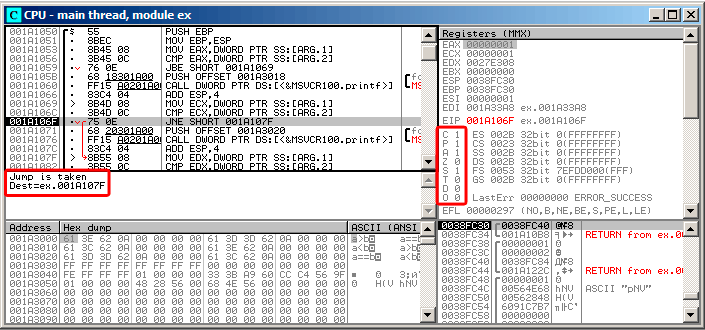
\includegraphics[scale=\FigScale]{patterns/07_jcc/simple/olly_unsigned2.png}
\caption{\olly: \TT{f\_unsigned()}: \RU{второй условный переход}\EN{second conditional jump}}
\label{fig:jcc_olly_unsigned_2}
\end{figure}

\olly \RU{подсказывает, что}\EN{gives a hint that} \JNZ \RU{сработает}\EN{is to be triggered now}.
\RU{Действительно}\EN{Indeed}, \JNZ \RU{срабатывает если}\EN{triggering if} ZF=0 (zero flag).

\clearpage
\RU{Третий переход,}\EN{The third conditional jump,} \JNB:

\begin{figure}[H]
\centering
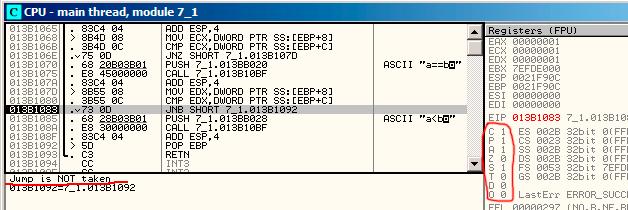
\includegraphics[scale=\FigScale]{patterns/07_jcc/simple/olly_unsigned3.png}
\caption{\olly: \TT{f\_unsigned()}: \RU{третий условный переход}\EN{third conditional jump}}
\label{fig:jcc_olly_unsigned_3}
\end{figure}

\RU{В}\EN{In} \cite{Intel} \RU{мы можем найти что}\EN{we can see that} \JNB \RU{срабатывает если}
\EN{triggers if} CF=0 (carry flag).
\RU{В нашем случае это не так, так что переход не срабатывает, и исполняется третий по счету}
\EN{It's not true in our case, so the third} \printf\EN{ executes}.

\clearpage
\RU{Теперь можно попробовать в \olly ф-цию}\EN{Now we can try in \olly the} \TT{f\_signed()} 
\RU{работающую с знаковыми величинами}\EN{function, which works with signed values}.

\RU{Флаги выставляются точно так же}\EN{Flags are set in the same way}: 
C=1, P=1, A=1, Z=0, S=1, T=0, D=0, O=0.

\RU{Первый переход}\EN{The first conditional jump} \JLE \RU{сработает}\EN{is to be triggered}:

\begin{figure}[H]
\centering
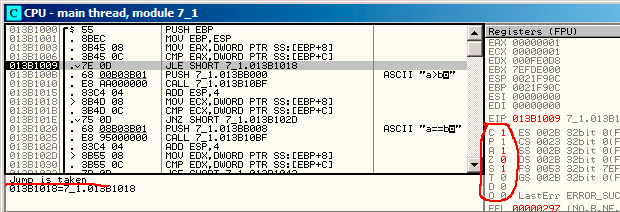
\includegraphics[scale=\FigScale]{patterns/07_jcc/simple/olly_signed1.png}
\caption{\olly: \TT{f\_unsigned()}: \RU{первый условный переход}\EN{first conditional jump}}
\label{fig:jcc_olly_signed_1}
\end{figure}

\RU{В}\EN{In} \cite{Intel} \RU{мы можем прочитать что эта инструкция срабатывает если}\EN{we find
that this instruction is triggered if} 
ZF=1 \OrENRU SF$\neq$OF.
\RU{В нашем случае, }SF$\neq$OF\RU{, так что переход срабатывает}\EN{ in our case, so the jump triggers}.

\clearpage
\RU{Второй переход}\EN{The second} \JNZ \RU{сработает}\EN{conditional jump triggering}: 
\RU{он срабатывает если}\EN{if} ZF=0 (zero flag):

\begin{figure}[H]
\centering
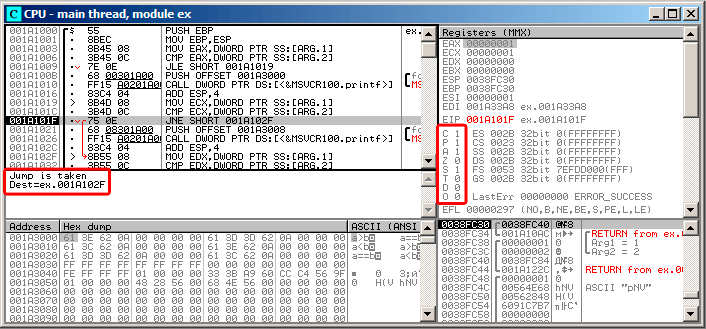
\includegraphics[scale=\FigScale]{patterns/07_jcc/simple/olly_signed2.png}
\caption{\olly: \TT{f\_unsigned()}: \RU{второй условный переход}\EN{second conditional jump}}
\label{fig:jcc_olly_signed_2}
\end{figure}

\clearpage
\RU{Третий переход}\EN{The third conditional jump} \JGE 
\RU{не сработает, потому что он срабатывает только если}
\EN{will not trigger because it will only if} SF=OF, 
\RU{что в нашем случае не так}\EN{and that is not true in our case}:

\begin{figure}[H]
\centering
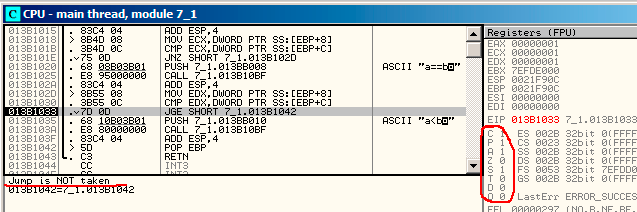
\includegraphics[scale=\FigScale]{patterns/07_jcc/simple/olly_signed3.png}
\caption{\olly: \TT{f\_unsigned()}: \RU{третий условный переход}\EN{third conditional jump}}
\label{fig:jcc_olly_signed_3}
\end{figure}

\fi

\clearpage
\subsubsection{x86 + MSVC + Hiew}
\index{Hiew}

\RU{Можем попробовать модифицировать исполняемый файл так,}\EN{We can try to patch the executable file in a way} 
\RU{чтобы функция}\EN{that the} \TT{f\_unsigned()} \RU{всегда показывала}\EN{function would always print} ``a==b'', 
\RU{при любых входящих значениях}\EN{no matter the input values}.
\RU{Вот как она выглядит в}\EN{Here is how it looks in} Hiew:

\begin{figure}[H]
\centering
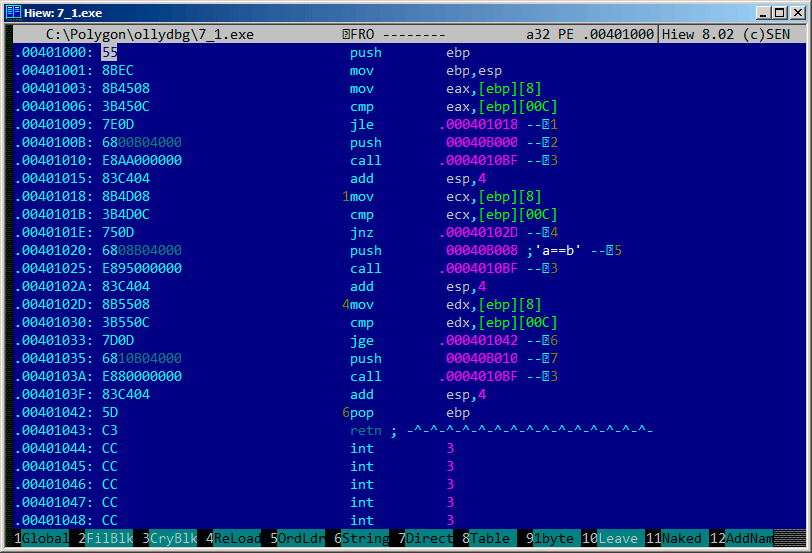
\includegraphics[scale=\FigScale]{patterns/07_jcc/simple/hiew_unsigned1.png}
\caption{Hiew: \RU{функция }\TT{f\_unsigned()}\EN{ function}}
\label{fig:jcc_hiew_1}
\end{figure}

\RU{Собственно, задач три}\EN{Essentially, we need to accomplish three tasks}:
\begin{itemize}
\item \RU{заставить первый переход срабатывать всегда}\EN{force the first jump to always trigger};
\item \RU{заставить второй переход не срабатывать никогда}\EN{force the second jump to never trigger};
\item \RU{заставить третий переход срабатывать всегда}\EN{force the third jump to always trigger}.
\end{itemize}

\RU{Так мы направим путь исполнения кода (code flow) во второй}\EN{Thus we can direct the code flow
to always pass through the second} \printf,
\RU{и он всегда будет срабатывать и выводить на консоль}\EN{and output} ``a==b''.

\RU{Для этого нужно изменить три инструкции (или байта)}\EN{Three instructions (or bytes) has to be patched}:

\begin{itemize}
\item \RU{Первый переход теперь будет}\EN{The first jump becomes} \JMP, \RU{но смещение перехода 
(\gls{jump offset}) останется прежним}\EN{but the \gls{jump offset} would remain the same}.

\item \RU{Второй переход может быть и будет срабатывать иногда, но в любом случае он будет совершать переход
только на следующую инструкцию, потому что мы выставляем смещение перехода (\gls{jump offset}) в 0.}
\EN{The second jump might be triggered sometimes, but in any case it will jump to the next
instruction, because, we set the \gls{jump offset} to 0.}
\RU{В этих инструкциях смещение перехода просто прибавляется к адресу следующей инструкции.}
\EN{In these instructions the \Gls{jump offset} is added to the address for the next instruction.}
\RU{Когда смещение 0, переход будет на следующую инструкцию.}\EN{So if the offset is 0,
the jump will transfer the control to the next instruction.}

\item \RU{Третий переход конвертируем в \JMP точно так же, как и первый, он будет срабатывать всегда.}
\EN{The third jump we replace with \JMP just as we do with the first one, so it will always trigger.}

\end{itemize}

\clearpage
\RU{Что и делаем}\EN{Here is the modified code}:

\begin{figure}[H]
\centering
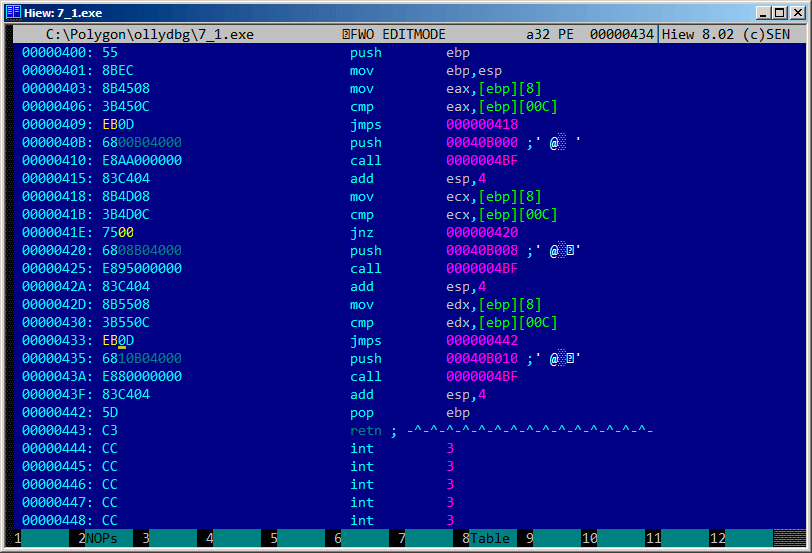
\includegraphics[scale=\FigScale]{patterns/07_jcc/simple/hiew_unsigned2.png}
\caption{Hiew: \RU{модифицируем функцию}\EN{let's modify the} \TT{f\_unsigned()}\EN{ function}}
\label{fig:jcc_hiew_2}
\end{figure}

\RU{Если забыть про какой-то из переходов, то тогда будет срабатывать несколько вызовов \printf, 
а нам ведь нужно чтобы исполнялся только один.}
\EN{If we miss to change any of these jumps, then several \printf calls may execute, while we want to execute only one.}

\ifdefined\IncludeGCC
\subsubsection{\NonOptimizing GCC}

\index{puts() \RU{вместо}\EN{instead of} printf()}
\NonOptimizing GCC 4.4.1 \RU{производит почти такой же код, за исключением}
\EN{produces almost the same code, but with} \puts~(\myref{puts}) \RU{вместо}\EN{instead of} \printf.

\subsubsection{\Optimizing GCC}

\RU{Наблюдательный читатель может спросить, зачем исполнять \CMP так много раз,
если флаги всегда одни и те же}\EN{An observant reader may ask, why execute \CMP several times, 
if the flags has the same values after each execution}?
\RU{По видимому, оптимизирующий MSVC не может этого делать, но GCC 4.8.1 делает больше оптимизаций:}
\EN{Perhaps optimizing MSVC can not do this, but optimizing GCC 4.8.1 can go deeper:}

\lstinputlisting[caption=GCC 4.8.1 f\_signed()]{patterns/07_jcc/simple/GCC_O3_signed.asm}

% should be here instead of 'switch' section?
\RU{Мы здесь также видим}\EN{We also see} \TT{JMP puts} \RU{вместо}\EN{here instead of} \TT{CALL puts / RETN}.
\RU{Этот прием описан немного позже}%
\EN{This kind of trick will have explained later}: \myref{JMP_instead_of_RET}.

\RU{Нужно сказать, что x86-код такого типа редок}\EN{This type of x86 code 
is somewhat rare}.
MSVC 2012\RU{, как видно, не может генерировать подобное}\EN{ as it seems, can't generate such code}.
\RU{С другой стороны, программисты на ассемблере прекрасно осведомлены о том, что инструкции}\EN{On the other hand, assembly language programmers are fully aware of the fact that} \TT{Jcc} \RU{можно располагать последовательно.}
\EN{instructions can be stacked.}
\RU{Так что если вы видите это где-то, имеется немалая вероятность, что этот фрагмент кода был написан вручную.}
\EN{So if you see such stacking somewhere, it is highly probable that the code was hand-written.}

\EN{The}\RU{Функция} \TT{f\_unsigned()} \RU{получилась не настолько эстетически короткой}\EN{function is not that 
\ae{}sthetically short}:

\lstinputlisting[caption=GCC 4.8.1 f\_unsigned()]{patterns/07_jcc/simple/GCC_O3_unsigned.asm.\LANG}

\RU{Тем не менее, здесь 2 инструкции \TT{CMP} вместо трех.}
\EN{Nevertheless, there are two \TT{CMP} instructions instead of three.}
\RU{Так что, алгоритмы оптимизации GCC 4.8.1, наверное, ещё пока не идеальны.}
\EN{So optimization algorithms of GCC 4.8.1 are probably not perfect yet.} 
\fi
